\subsubsection{System Topologie}
\begin{figure}[H]
\centering
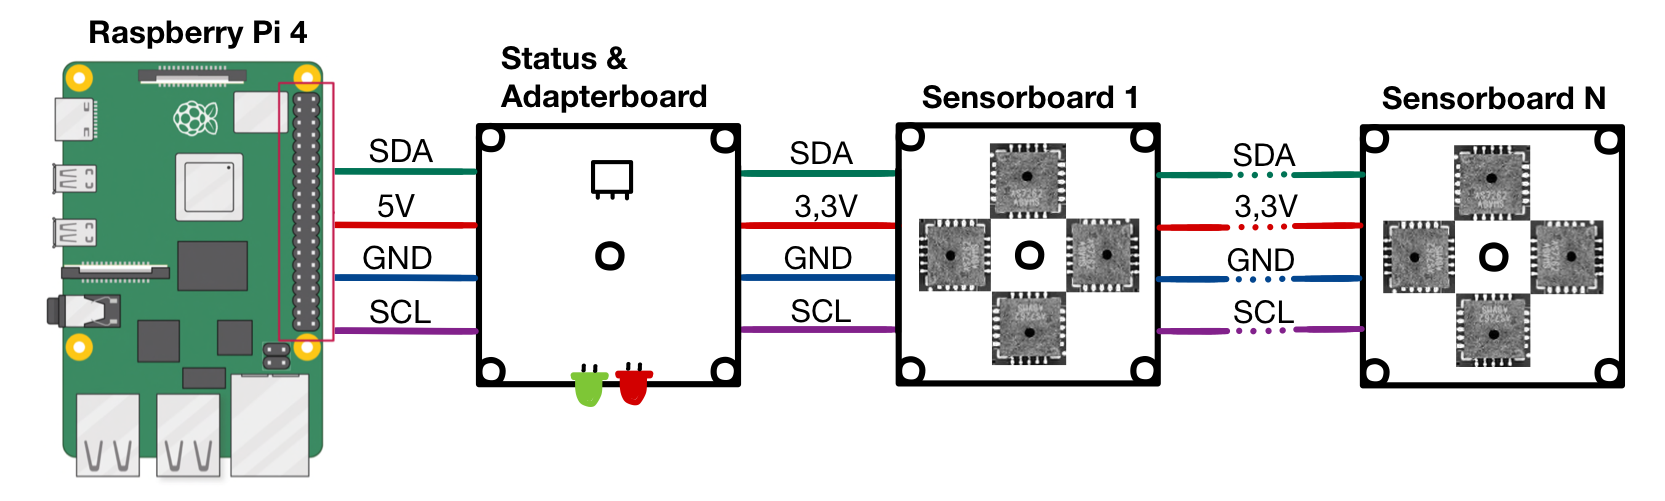
\includegraphics[width=1\textwidth]{img/System-Topologie.png}
%\caption*{Quelle: Datenblatt AS7261}
\caption{Verschaltung der der Platienen}
\label{fig:Seitenasicht-AS726X}
\end{figure}
\subsubsection{Status \& Adapterboard}
Da der NanoPi nicht die benötigte $3,3V$ Stromversorgung bereitstellt wird eine Adapter-Shield mit einem Spannungswandler(LM3940IT-3.3) verwendet.
Auf dem Adapter-Shield findet der einheitliche Steckverbinder Platz, da das Adapter-Shield aufgrund seiner Bauform nicht falsch montiert werden kann so die Verpolung der Sensoren ausgeschlossen werden.
Die Bedeutung der Status LED wird im Handbuch \ref{todo} erläutert.\\

\begin{figure}[H]
\centering
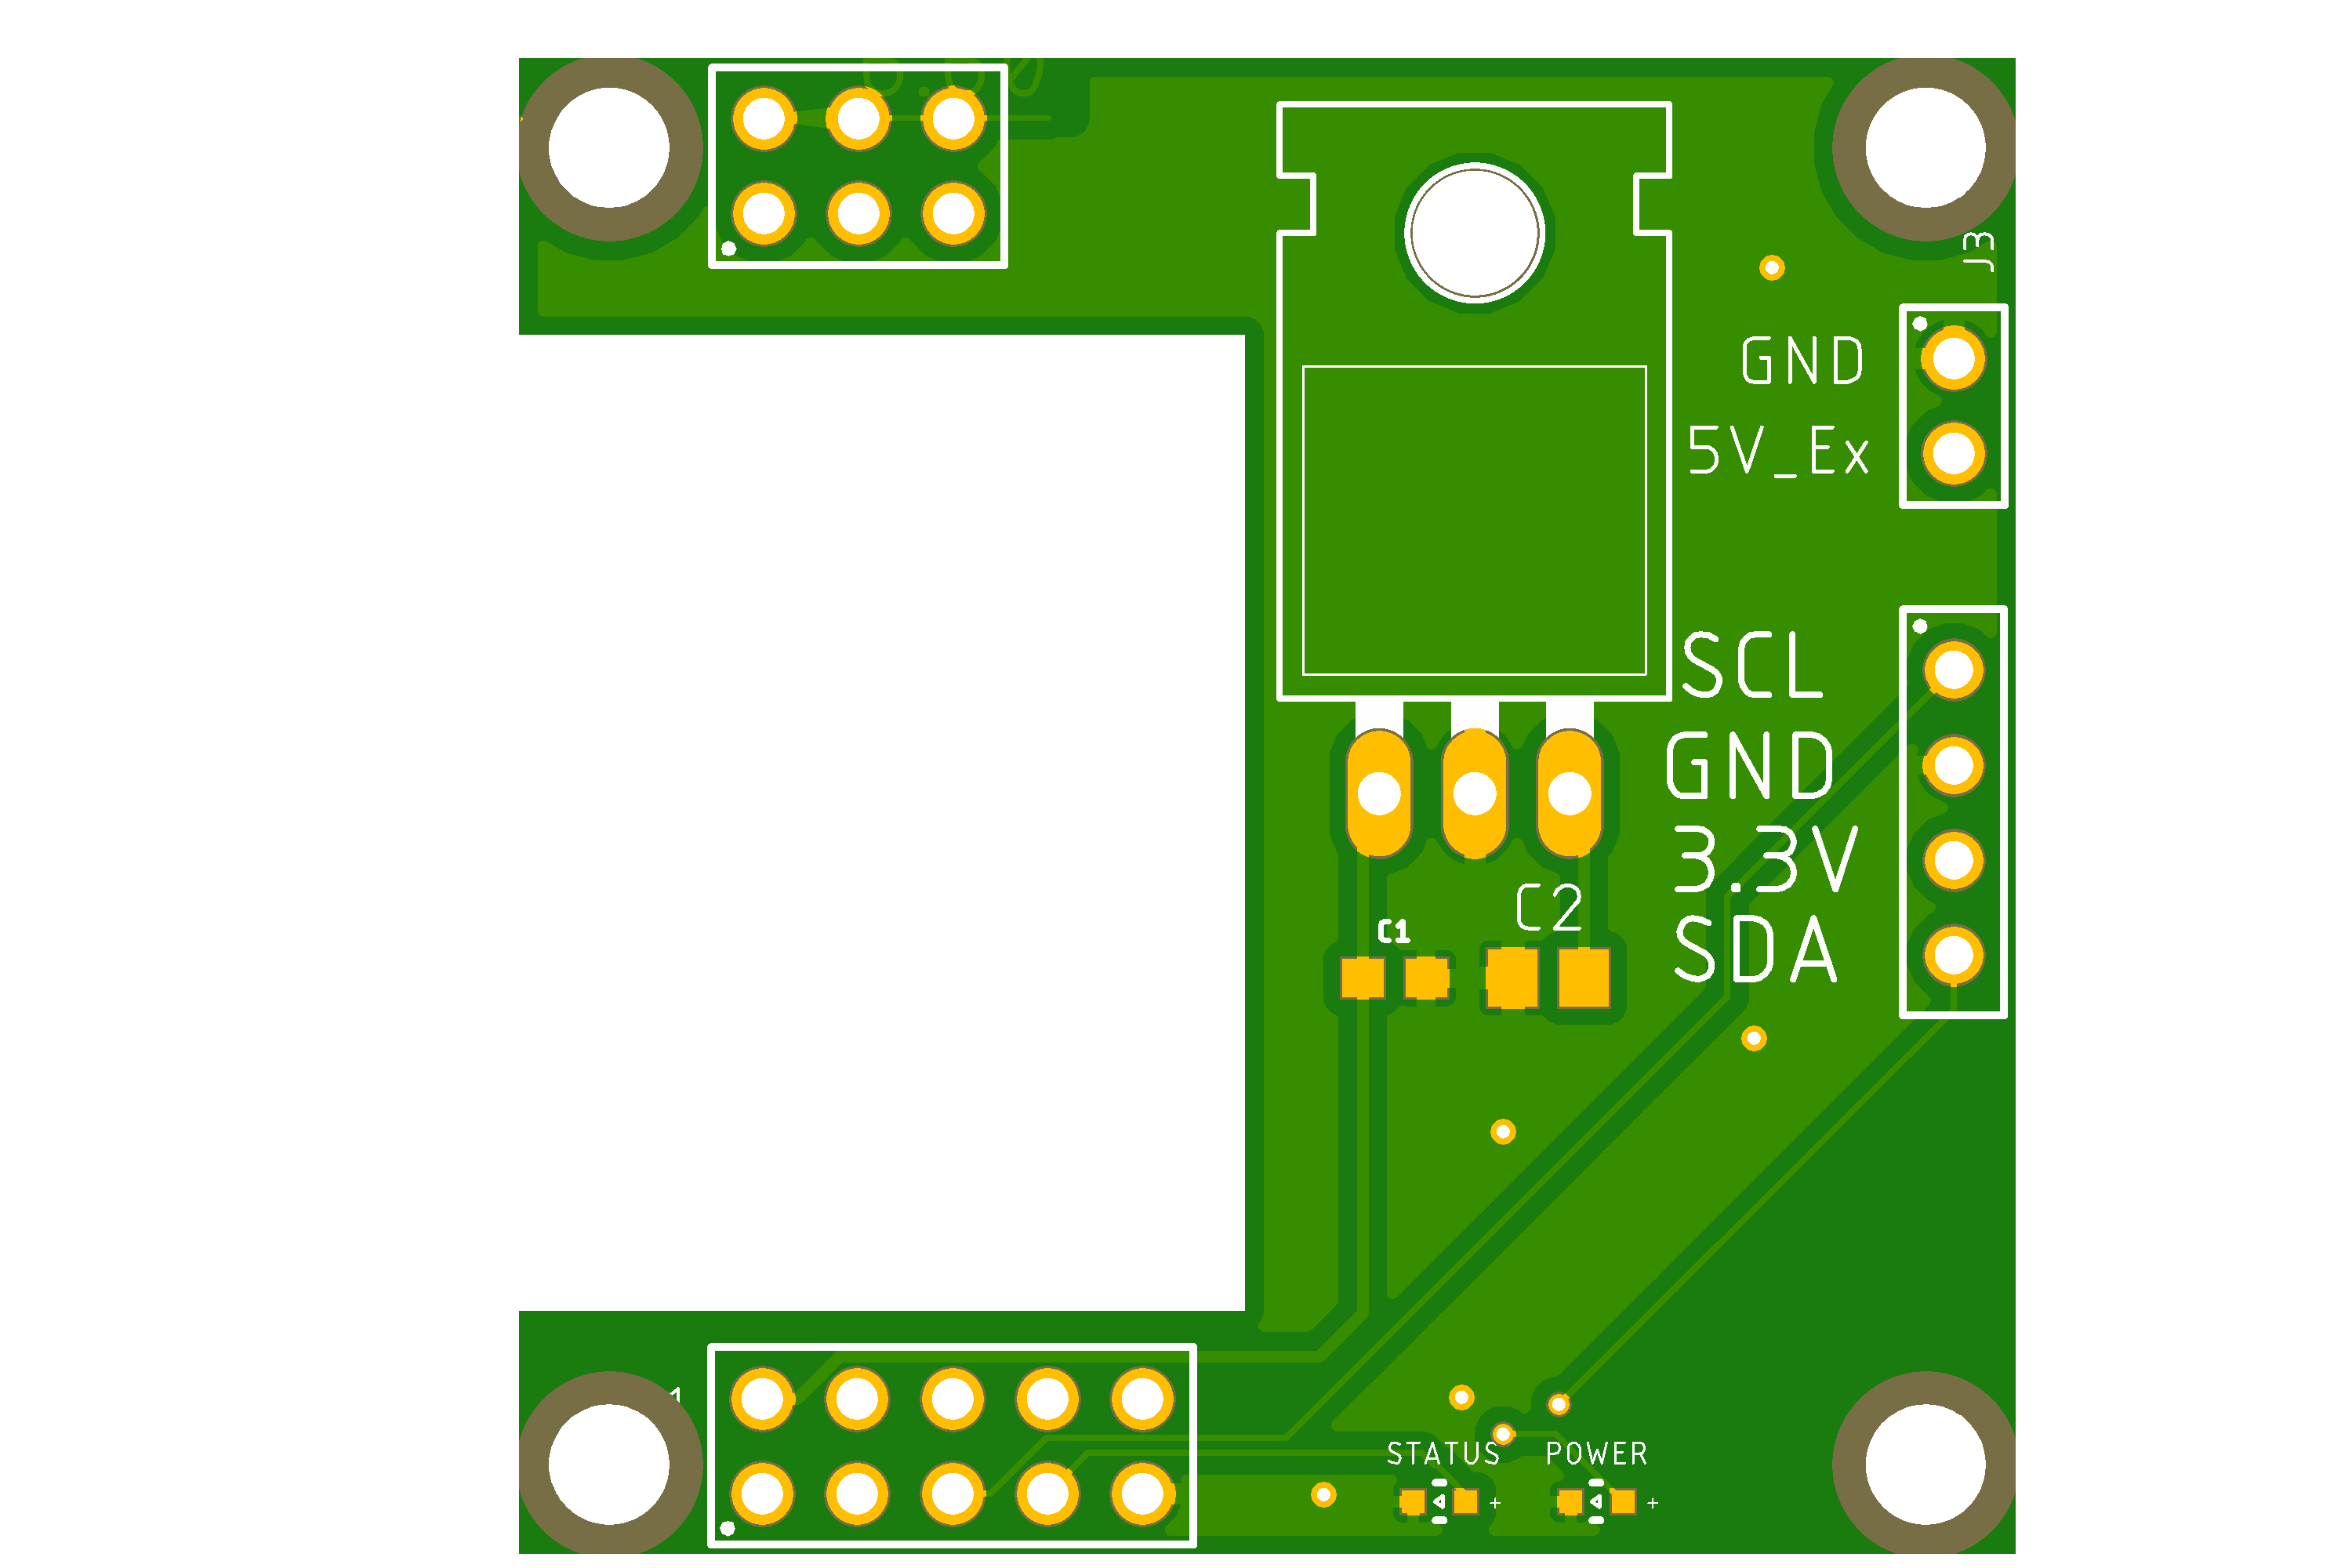
\includegraphics[width=0.75\textwidth]{img/nanopi-black2-shield}
%\caption*{Quelle: Datenblatt AS7261}
\caption{Verschaltung der der Platienen}
\label{fig:Seitenasicht-AS726X}
\end{figure}

\subsubsection{Sensorboard}
\begin{figure}[H]
\centering
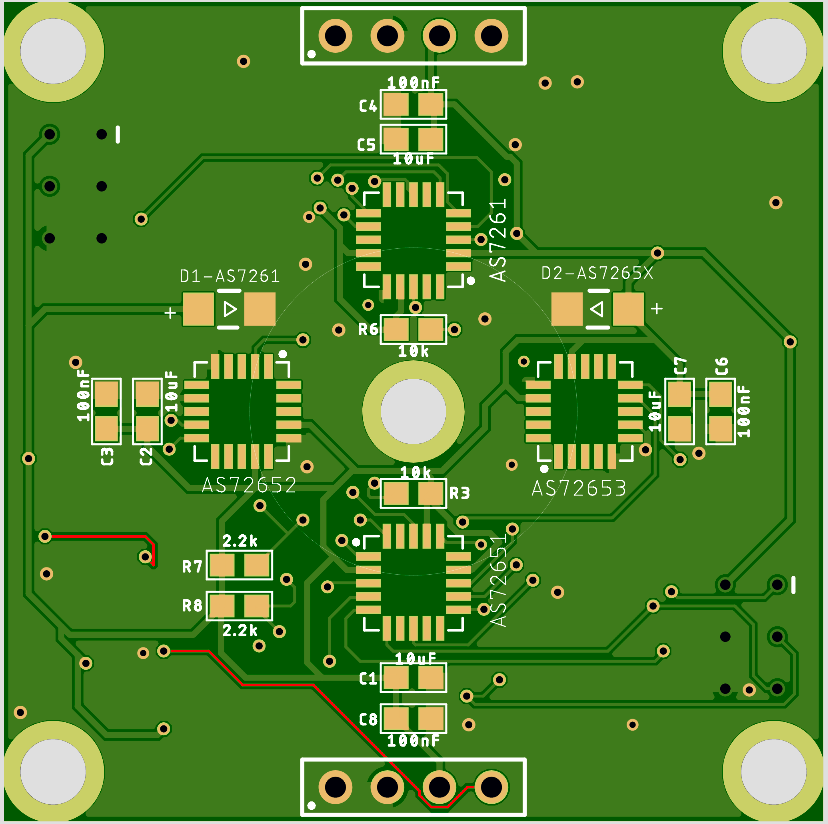
\includegraphics[width=0.75\textwidth]{img/Sensor-platiene_front}
%\caption*{Quelle: Datenblatt AS7261}
\caption{Verschaltung der der Platienen}
\label{fig:Seitenasicht-AS726X}
\end{figure}

\begin{figure}[H]
\centering
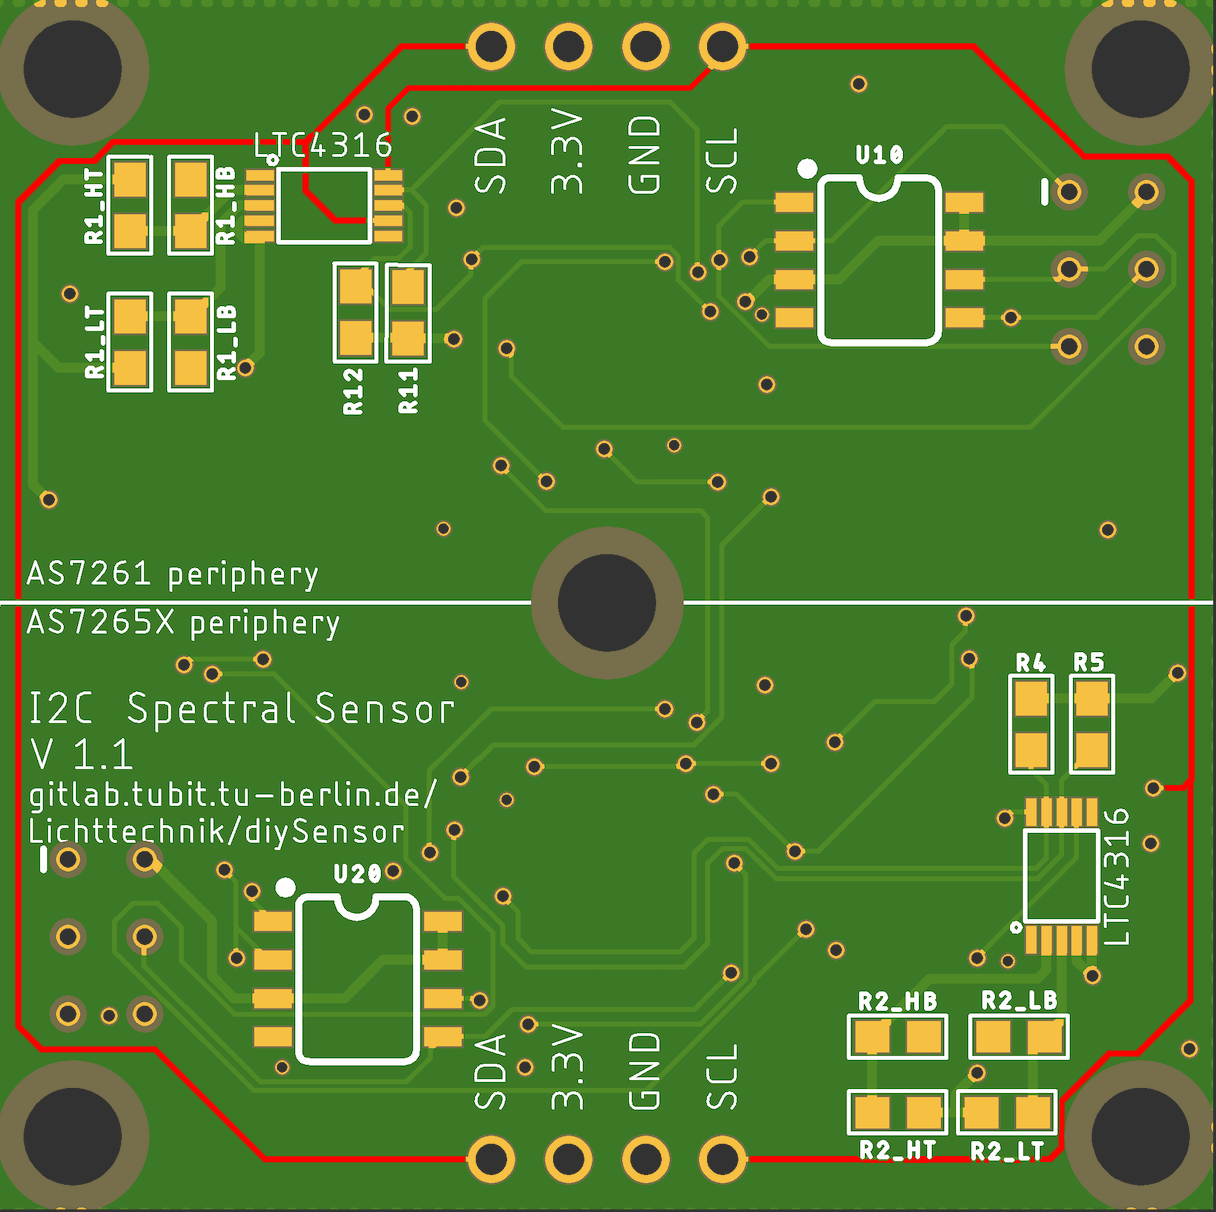
\includegraphics[width=0.75\textwidth]{img/Sensor-platiene_back}
%\caption*{Quelle: Datenblatt AS7261}
\caption{Verschaltung der der Platienen}
\label{fig:Seitenasicht-AS726X}
\end{figure}